\documentclass{beamer}

\usepackage[utf8]{inputenc}
\usepackage[T1]{fontenc}
\usepackage{booktabs}
\usepackage{bm}

% page numbering
\setbeamertemplate{footline}[frame number]{}
\setbeamerfont{footline}{size=\large}

% remove navigation symbols
\beamertemplatenavigationsymbolsempty

% remove caption prefix
\setbeamertemplate{caption}{\raggedright\insertcaption\par}

\title{Reproducing \textit{Colorful Image Colorization}}
\author{Timo Nicolai \and Álvaro Orgaz Expósito \and Carolina Bianchi}

\begin{document}

\begin{frame}[noframenumbering,plain]
  \titlepage
\end{frame}

% --- INTRODUCTION -------------------------------------------------------------

\begin{frame}{Introduction (I)}
  \textbf{Problem statement:}
    \begin{itemize}
      \item Infer colours given a grayscale image
      \item Ill-posed problem due to inherent multimodality \\
            $\rightarrow$ network should predict per-pixel colour distributions \\
            $\rightarrow$ produce \textit{plausible} colourization
    \end{itemize}

  \medskip

  \begin{figure}[!htb]
    \minipage{0.28\textwidth}
      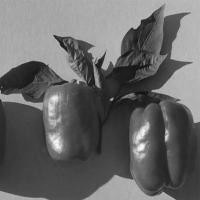
\includegraphics[width=\linewidth]{resources/bw.jpg}
      \caption{Input}
    \endminipage\hfill
    \minipage{0.28\textwidth}
      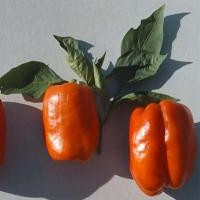
\includegraphics[width=\linewidth]{resources/gt.jpg}
      \caption{Ground truth}
    \endminipage\hfill
    \minipage{0.28\textwidth}%
      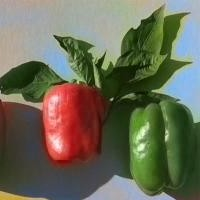
\includegraphics[width=\linewidth]{resources/colored.jpg}
      \caption{Colourized}
    \endminipage
  \end{figure}
\end{frame}

\begin{frame}{Introduction (II)}
  \textbf{Applications:}
    \begin{itemize}
        \item Colourization of historical images
        \item Preprocessing step in grayscale image classification
        \item Representation learning for transfer learning tasks
    \end{itemize}
\end{frame}

% --- RELATED WORK -------------------------------------------------------------

\begin{frame}{Related work (I)}
  \textbf{Early approaches to the problem:}

    \medskip

    \begin{itemize}
      \item Synthesise colours from reference pictures (Welsh et al., 2002)

      \begin{figure}[!htb]
        \minipage{0.50\textwidth}
          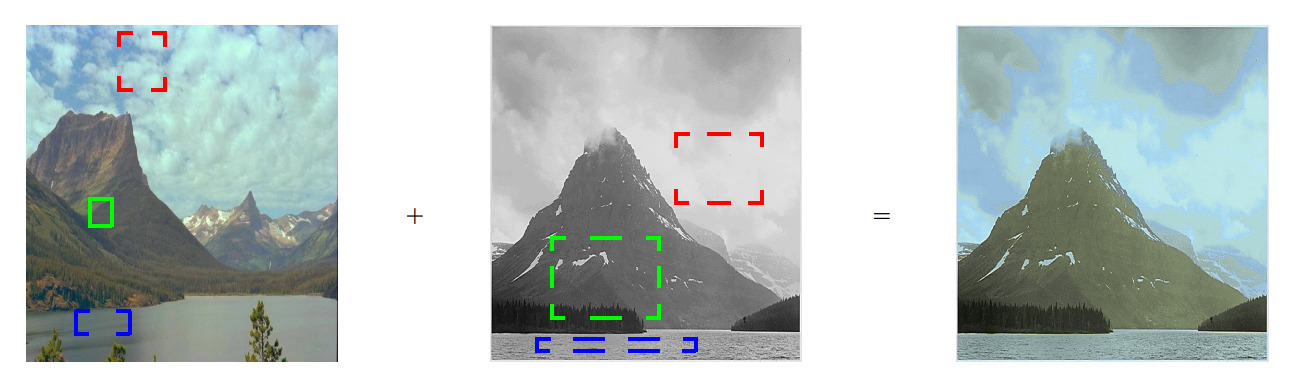
\includegraphics[width=\linewidth]{resources/welsh.jpg}
        \endminipage
      \end{figure}

      \medskip

      \item Colourization as an optimization problem (Levin et al., 2004)

      \begin{figure}[!htb]
        \minipage{0.50\textwidth}
          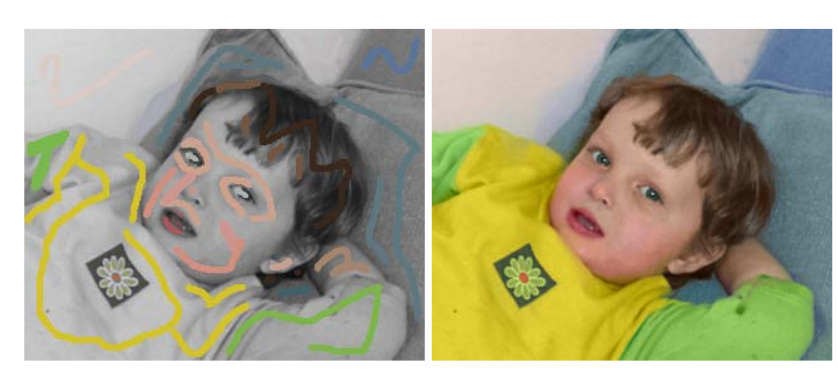
\includegraphics[width=\linewidth]{resources/levin.jpg}
        \endminipage
      \end{figure}
    \end{itemize}
\end{frame}

\begin{frame}{Related work (II)}
  \textbf{Modern approaches:}
    \begin{itemize}
      \item Leverage large-scale data: deep learning approaches with different
            architectures and cost functions (Larsson et al. 2016,
            Iizuka et al. 2016, \textbf{Zhang et al. 2016})
      \item Use Generative Adversarial Network to automatically learn the cost
            function (Nazeri et al. 2018)
      \item Exemplar-based colourization with automatic reference retrieval
            (He et al. 2018)
    \end{itemize}
\end{frame}

% --- DATA ---------------------------------------------------------------------

\begin{frame}{Data (I)}
  \begin{itemize}
    \item Analyze images in the L*a*b* colour space \\
          $\rightarrow$ Use L channel as input \\
          $\rightarrow$ Use a and b channel as supervisory signals
    \item Resize images to 256x256 px
    \item Randomly crop images to 176x176 px during training
  \end{itemize}

  \medskip

  \begin{figure}[!htb]
    \minipage{0.24\textwidth}
      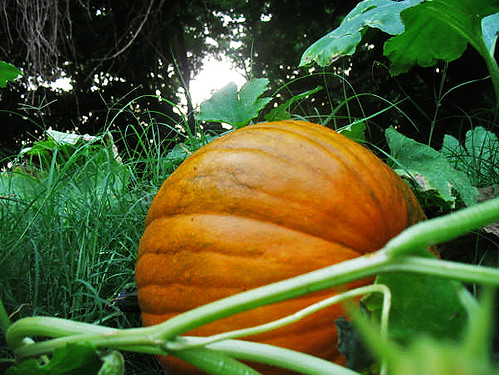
\includegraphics[width=\linewidth]{resources/pumpkin.jpg}
      \caption{Original}
    \endminipage\hfill
    \minipage{0.24\textwidth}
      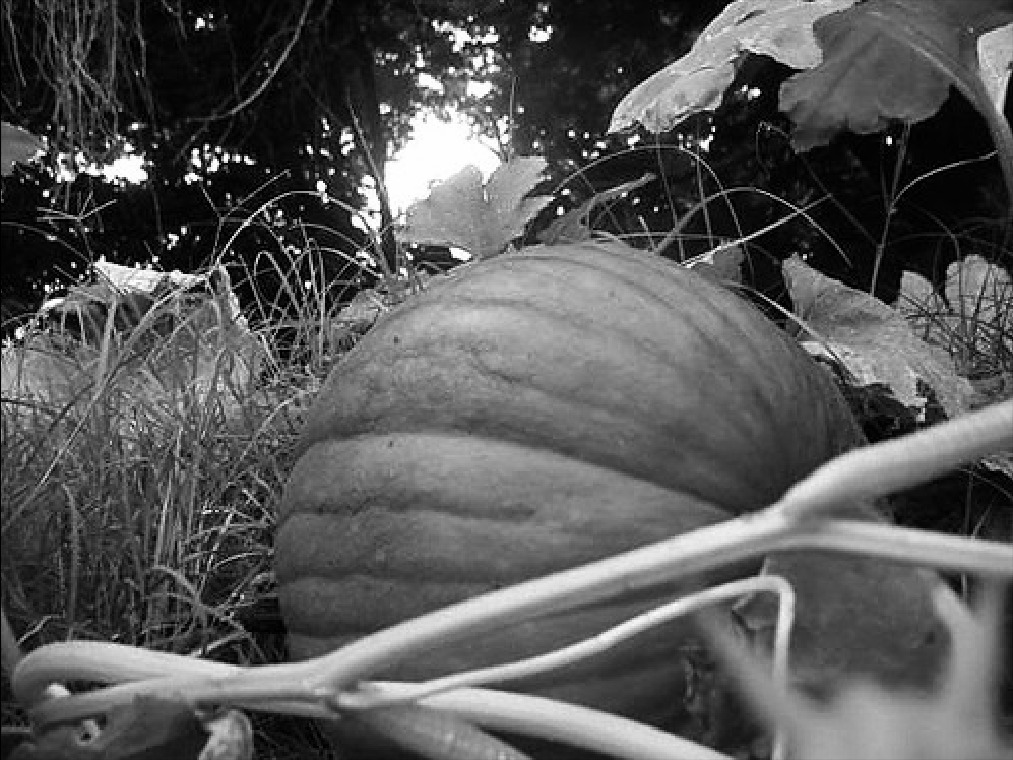
\includegraphics[width=\linewidth]{resources/pumpkin_bw.jpg}
      \caption{L channel}
    \endminipage\hfill
    \minipage{0.24\textwidth}
      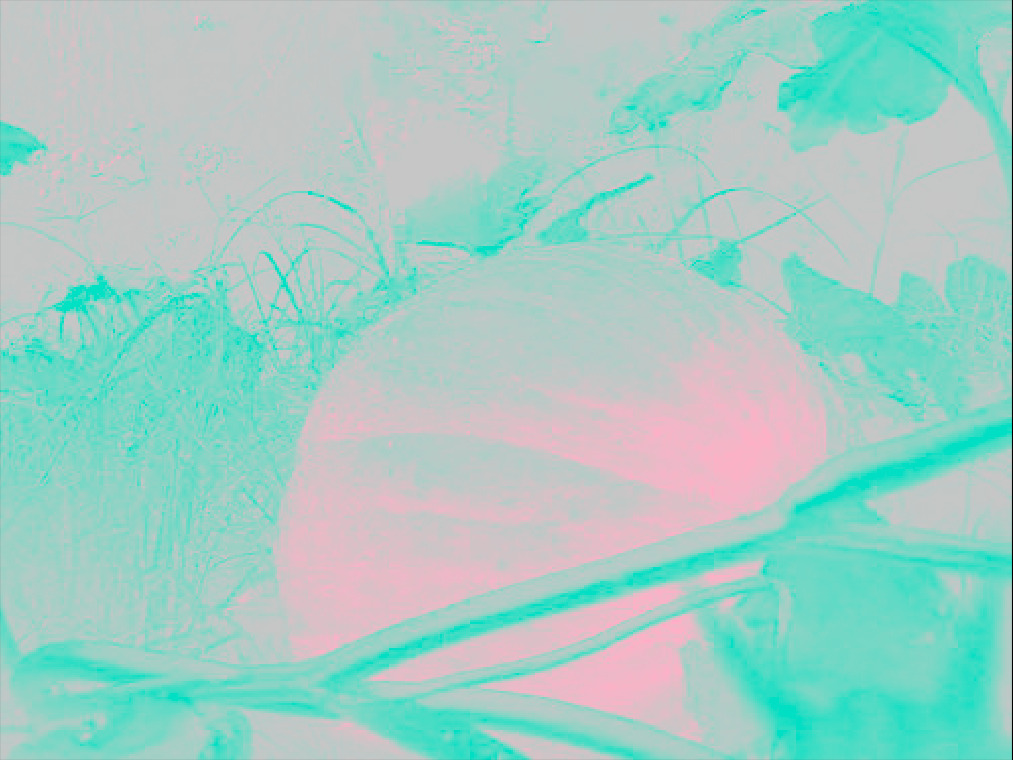
\includegraphics[width=\linewidth]{resources/pumpkin_a.jpg}
      \caption{a channel}
    \endminipage\hfill
    \minipage{0.24\textwidth}
      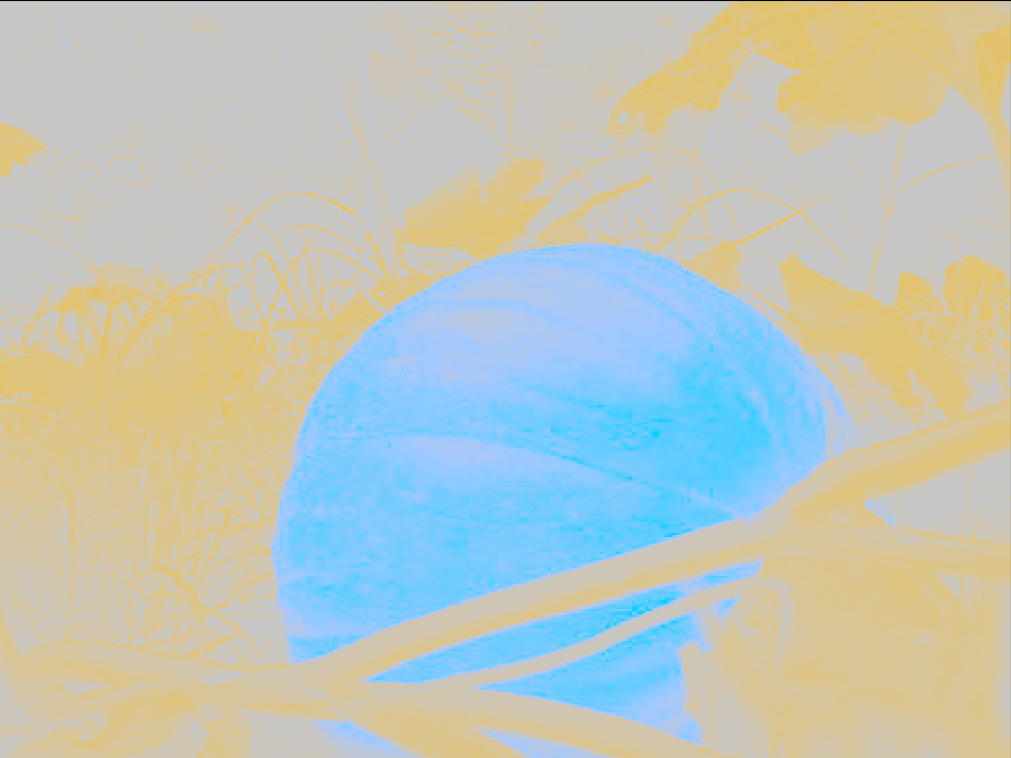
\includegraphics[width=\linewidth]{resources/pumpkin_b.jpg}
      \caption{b channel}
    \endminipage
  \end{figure}
\end{frame}

\begin{frame}{Data (II)}
  \textbf{Dataset:}
    \begin{itemize}
      \item Subset of ImageNet (42.566 images)
      \item Semantically related categories (mostly fruits and vegetables) \\
            $\rightarrow$ Make training feasible given computational resources \\
            $\rightarrow$ Vibrant colours: easy to inspect quality of the results
    \end{itemize}

  \medskip

  \begin{figure}
    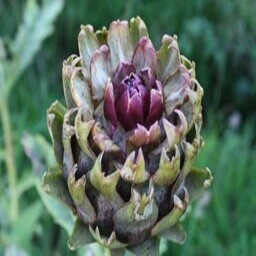
\includegraphics[width=.23\linewidth]{resources/veg1.jpg}\hfill
    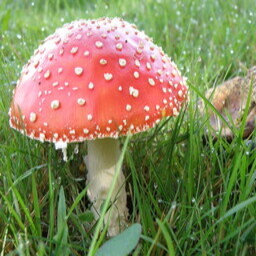
\includegraphics[width=.23\linewidth]{resources/veg2.jpg}\hfill
    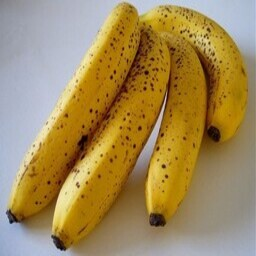
\includegraphics[width=.23\linewidth]{resources/veg3.jpg}\hfill
    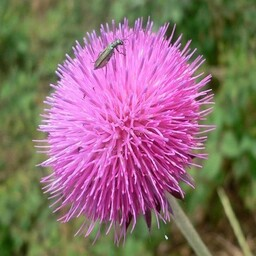
\includegraphics[width=.23\linewidth]{resources/veg4.jpg}
    \caption{Examples of images from our training set}
  \end{figure}
\end{frame}

% --- METHODS ------------------------------------------------------------------

\begin{frame}{Methods (I): Network Output}
  \textbf{Input:}
    \begin{itemize}
       \item Luminance channel $L$
    \end{itemize}

  \medskip

  \textbf{Target:}
    \begin{itemize}
      \item Discrete, in-gamut $ab$ output space with $Q = 313$ bins
    \end{itemize}

  \medskip

  \begin{center}
    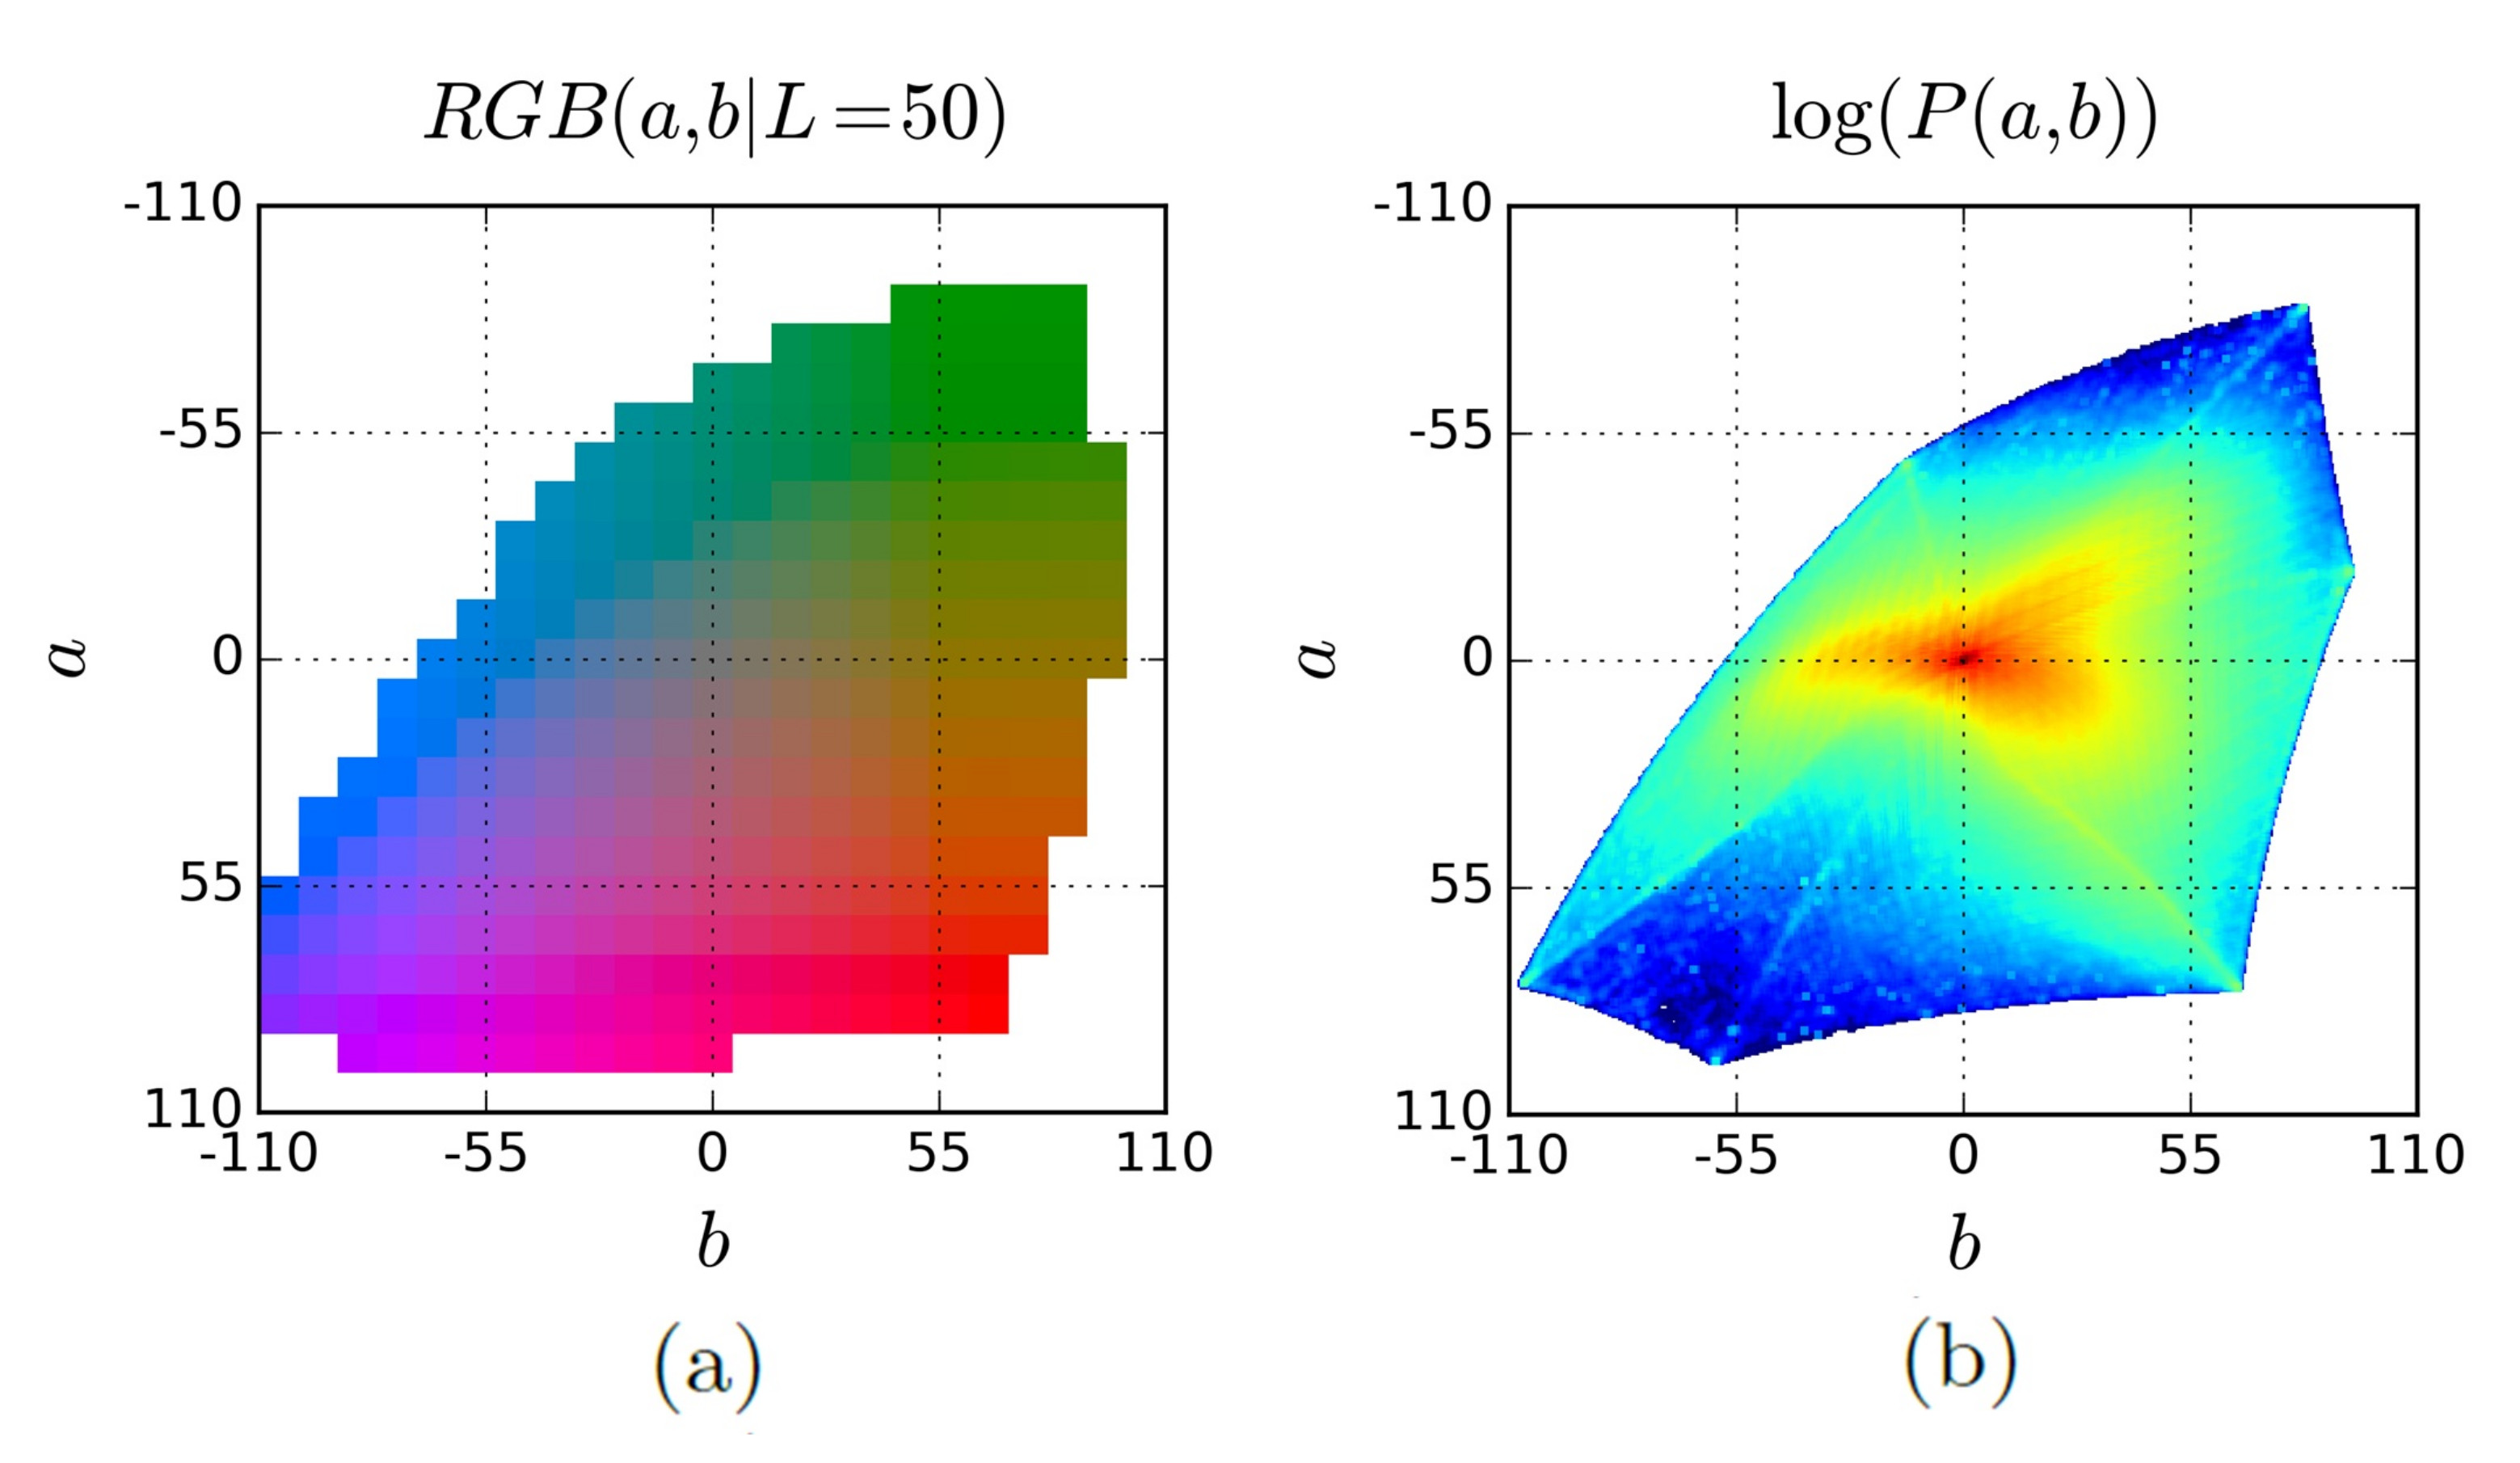
\includegraphics[width=.4\linewidth]{resources/gamut.jpg}
  \end{center}
\end{frame}

\begin{frame}{Methods (II): Loss Function}
  \begin{itemize}
    \item Raw output: probability distribution $\hat{Z} \in [0, 1]^{H \times W \times Q}$
    \item Obtain $Z$ from ground truth via \textbf{soft encoding}
  \end{itemize}

  \begin{equation}
    L(Z, \hat{Z}) = -\sum_{w,h} v(Z_{w,h}) \sum_q Z_{w,h,q} \cdot log(\hat{Z}_{w,h,q})
  \end{equation}

  \begin{itemize}
    \item Use \textbf{class rebalancing} to achieve plausible colourizations
  \end{itemize}

  \begin{equation}
    v(Z_{w,h}) \propto \left((1 - \lambda) \tilde{\bm{p}} + \frac{\lambda}{Q} \right)^{-1}
  \end{equation}

  \begin{itemize}
    \item $\tilde{\bm{p}}$ is prior distribution (from ImageNet training set)
  \end{itemize}
\end{frame}

\begin{frame}{Methods (III): From Colour Probabilities to Point Estimates}
  \begin{itemize}
    \item Decode $\hat{Z}$ to $ab \in [-110,110]^{H \times W \times 2}$ via \textbf{Annealed Mean}
  \end{itemize}

  \begin{equation}
    H(Z_{h,w}) = E[f(Z_{h,w})] \qquad f(z) = \frac{exp(log(z)/T)}{\sum_q exp(log(z)/T)}
  \end{equation}

  \begin{itemize}
    \item Can adjust \textbf{Temperature} parameter $T \in [1, 0)$ \\
          $\rightarrow$ lower $T$: higher vibrancy \\
          $\rightarrow$ higher $T$: higher spatial consistency
  \end{itemize}

  \medskip

  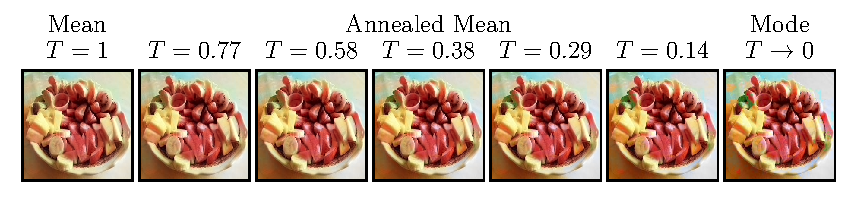
\includegraphics[width=\linewidth]{resources/annealed_mean.pdf}
\end{frame}

\begin{frame}{Methods (IV): Network Architecture}
  \textbf{Input data:}
    \begin{itemize}
       \item Luminance channel $L$
    \end{itemize}

  \medskip

  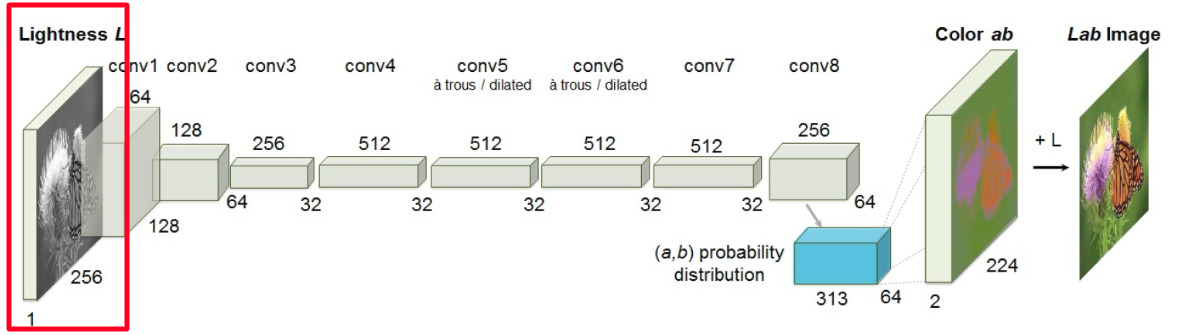
\includegraphics[width=\linewidth]{resources/network1.jpg}
\end{frame}

\begin{frame}{Methods (IV): Network Architecture}
  \textbf{Feature extraction:}
    \begin{itemize}
      \item VGG like network structure
      \item (atrous) convolution, deconvolution and batchnorm layers
      \item ReLU activations
      \item Kernel size $3 \times 3$
    \end{itemize}

  \medskip

  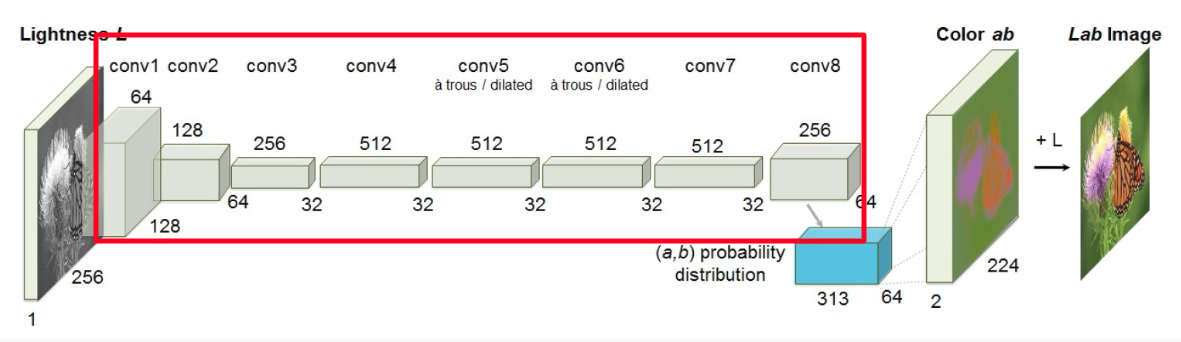
\includegraphics[width=\linewidth]{resources/network2.jpg}
\end{frame}

\begin{frame}{Methods (IV): Network Architecture}
  \textbf{Raw output:}
    \begin{itemize}
      \item Probability distribution $Z \in [0, 1]^{H \times W \times Q}$
    \end{itemize}

  \medskip

  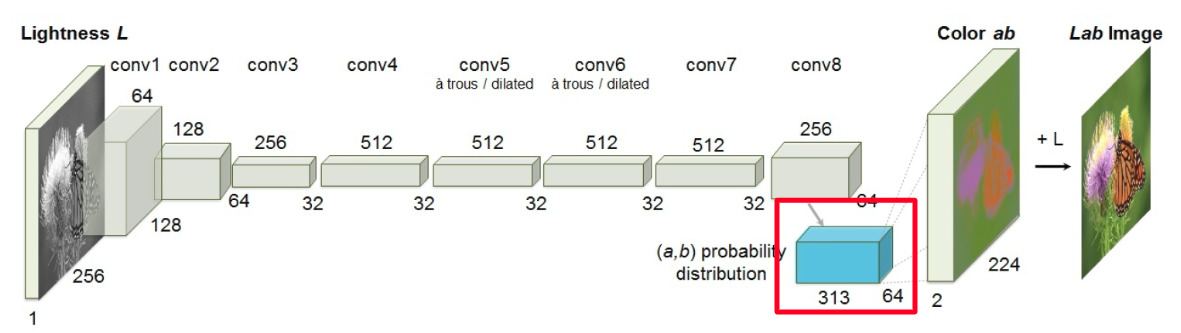
\includegraphics[width=\linewidth]{resources/network3.jpg}
\end{frame}

\begin{frame}{Methods (IV): Network Architecture}
  \textbf{Annealed mean:}
    \begin{itemize}
      \item $Z \in [0, 1]^{H \times W \times Q} \rightarrow ab \in [-110,110]^{H \times W \times 2}$
    \end{itemize}

  \medskip

  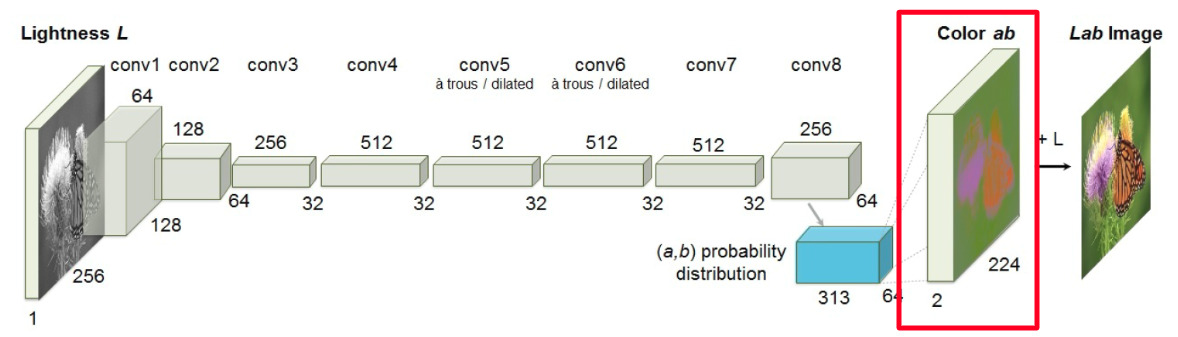
\includegraphics[width=\linewidth]{resources/network4.jpg}
\end{frame}

% --- EXPERIMENTS --------------------------------------------------------------

\begin{frame}{Training (I): Overview}
  \begin{center}
    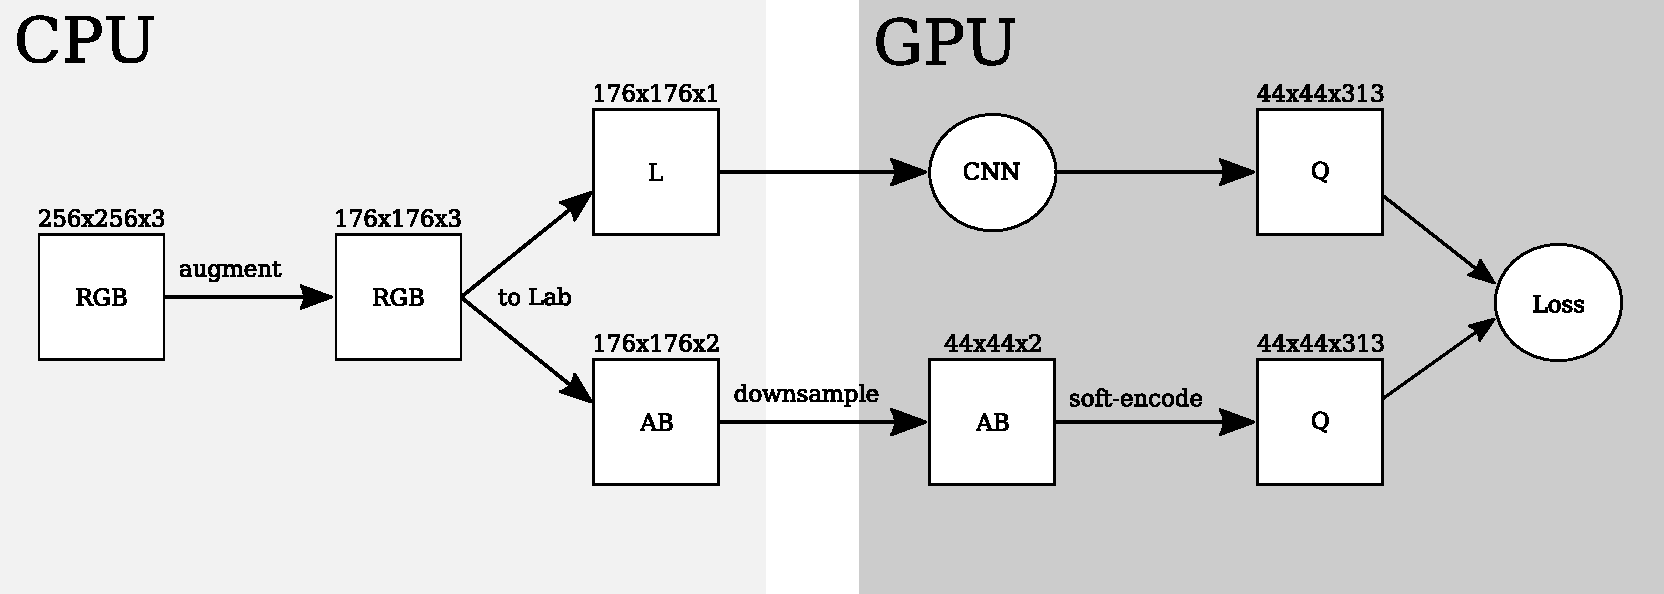
\includegraphics[width=\textwidth]{resources/training.pdf}
  \end{center}
\end{frame}

\begin{frame}{Training (II): Optimization}
  \begin{itemize}
    \item Adam optimizer
       \begin{itemize}
         \item $\beta_1 = .9$, $\beta_2 = .99$
         \item Weight decay = $10^-3$
         \item $\eta = 3.16 \time 10^{-5}$ (constant)
         \item Batch size = 40
       \end{itemize}
  \end{itemize}
\end{frame}

\begin{frame}{Training (III): Learning Curve}
  \begin{itemize}
    \item $\approx 20$ hours of training on NVIDIA Tesla V100
  \end{itemize}

  \begin{center}
    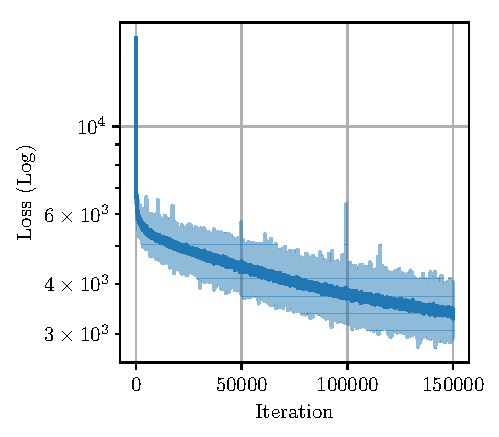
\includegraphics[width=.6\textwidth]{resources/learning_curve.pdf}
  \end{center}
\end{frame}

\begin{frame}{Examples}
  \begin{center}
    \includegraphics[height=.9\textheight]{resources/good_vs_bad_slides.pdf}
  \end{center}
\end{frame}

\begin{frame}{Perceptual Realism Study}
  \begin{center}
    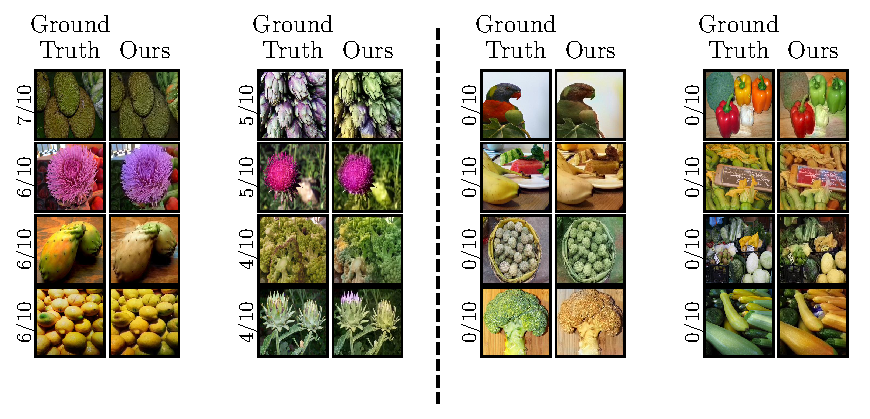
\includegraphics[width=\textwidth]{resources/amt_results_slides.pdf}
  \end{center}

  \begin{itemize}
    \item $50$ randomly chosen validation set images
    \item $10$ participants
    \item Fooled on average $18.78\%$ of the time
    \item Photorealistic results only for ``easy'' images
  \end{itemize}
\end{frame}

\begin{frame}{Colourization as Preprocessing (I)}
  \begin{center}
    \begin{tabular}{cc}
      \scalebox{0.8}{
        \begin{tabular}{ll}
          \toprule
          Method        & VGG-16 Top-5 Acc. \\
          \midrule
          Ground truth  & 92.1 \\
          Grayscale     & 46.4 \\
          Random colour & 17.4 \\
          \midrule
          Zhang et al.  & 67.7 \\
          Ours          & 81.0 \\
          \bottomrule
        \end{tabular}
      } & $\vcenter{\hbox{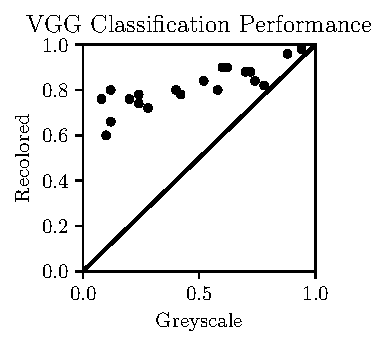
\includegraphics[width=.5\textwidth]{%
        resources/vgg_classification_performance.pdf}}}$
    \end{tabular}
  \end{center}

  \medskip

  \begin{itemize}
    \item Top-5 classification accuracy for 1000 validation set images
    \item $\rightarrow$ dramatically improved by colourization!
  \end{itemize}
\end{frame}

\begin{frame}{Colourization as Preprocessing (II)}
  \begin{columns}
    \begin{column}{0.4\textwidth}
      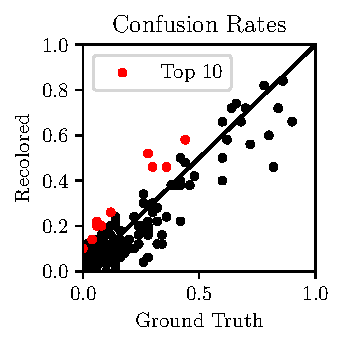
\includegraphics[width=\textwidth]{resources/confusion_rates.pdf}
    \end{column}
    \begin{column}{0.6\textwidth}
      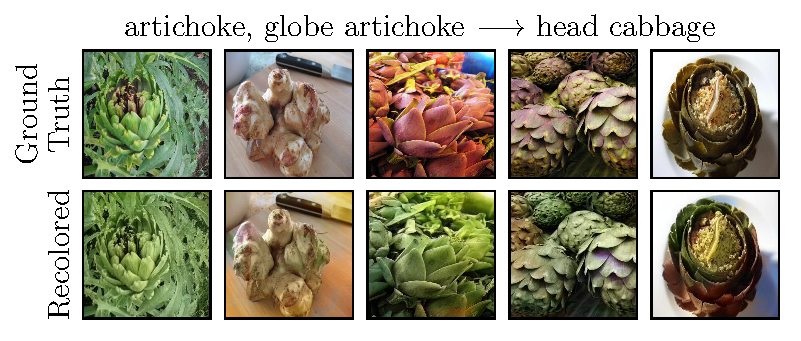
\includegraphics[width=\textwidth]{resources/common_confusions.pdf}
    \end{column}
  \end{columns}

  \medskip

  \begin{itemize}
    \item Colourization amplifies certain confusion cases
  \end{itemize}
\end{frame}

% --- CONCLUSIONS --------------------------------------------------------------

\begin{frame}{Conclusions}
  \begin{itemize}
    \item We successfully reproduced the results of Zhang et al. on a reduced dataset
    \item We showed how our network can improve grayscale image classification accuracy
    \item The network tends to miscolour background objects, future work might include: \\
      \begin{itemize}
        \item Exploring post-processing approaches that enforce spatial consistency
        \item Segmenting images into fore- and background and colouring them with
              separate networks
      \end{itemize}
  \end{itemize}
\end{frame}

% --- LEARNING OUTCOMES --------------------------------------------------------

\begin{frame}{Learning outcomes (I)}
  \textbf{Timo:}
    \begin{itemize}
      \item In-depth PyTorch skills, including implementing predefined
            architectures from common building blocks and implementing custom
            layers
      \item Increased familiarity with common CNN layers types, including
            (separable/transposed/atrous) convolutions, batch normalization,
            dropout etc.
      \item Deeper insight into the colourization problem: Lab colour space,
            input encoding and output decoding schemes, implementation and
            advantages of different loss functions and rebalancing schemes and
            how to assess colourization quality
    \end{itemize}
\end{frame}

\begin{frame}{Learning outcomes (II)}
  \textbf{Álvaro:}
    \begin{itemize}
      \item Deeper insight into the implementation of deep learning projects,
            concretely CNN concepts and image processing
      \item Useful programming skills, including PyTorch, remote Google
            computational resources, and Linux commands
      \item Customizing existing algorithms: preprocessing the target,
            customizing the loss function and obtaining the final prediction via
            an operation over the raw network output
    \end{itemize}
\end{frame}

\begin{frame}{Learning outcomes (III)}
  \textbf{Carolina:}
    \begin{itemize}
      \item Better knowledge of deep learning theory (CNN), techniques
            (PyTorch) and methodology
      \item Increased confidence with Google remote computing platforms
      \item Better understanding of the challenges involved in having to
            formulate the colourization problem in a computationally feasible
            way
    \end{itemize}
\end{frame}

\end{document}
